\subsection{Data Input}
\makesubcontentsslidessec

\begin{frame}
  \begin{block}{Parallel reading brings new issues}\pause
    \begin{itemize}
    \item How to partition data across nodes?
    \item How to structure for scalable libraries?
    \item Read directly into form needed or restructure?
    \end{itemize}
  \end{block}
  \begin{block}{Answers}\pause
    \begin{itemize}
    \item Read the most natural way from disk
      \begin{itemize}
      \item C: by blocks of rows
      \item FORTRAN: by blocks of columns
      \item Binary, fixed format, or groups of files
      \end{itemize}
    \item Restructure after reading
      \begin{itemize}
      \item redistribute(), as.ddmatrix(), etc.
      \end{itemize}
    \end{itemize}
  \end{block}
\end{frame}

\begin{frame}{Considering I/O Configurations}
\vspace{-1em}
  \begin{minipage}{0.32\textwidth}
    \begin{block}{Best!}
      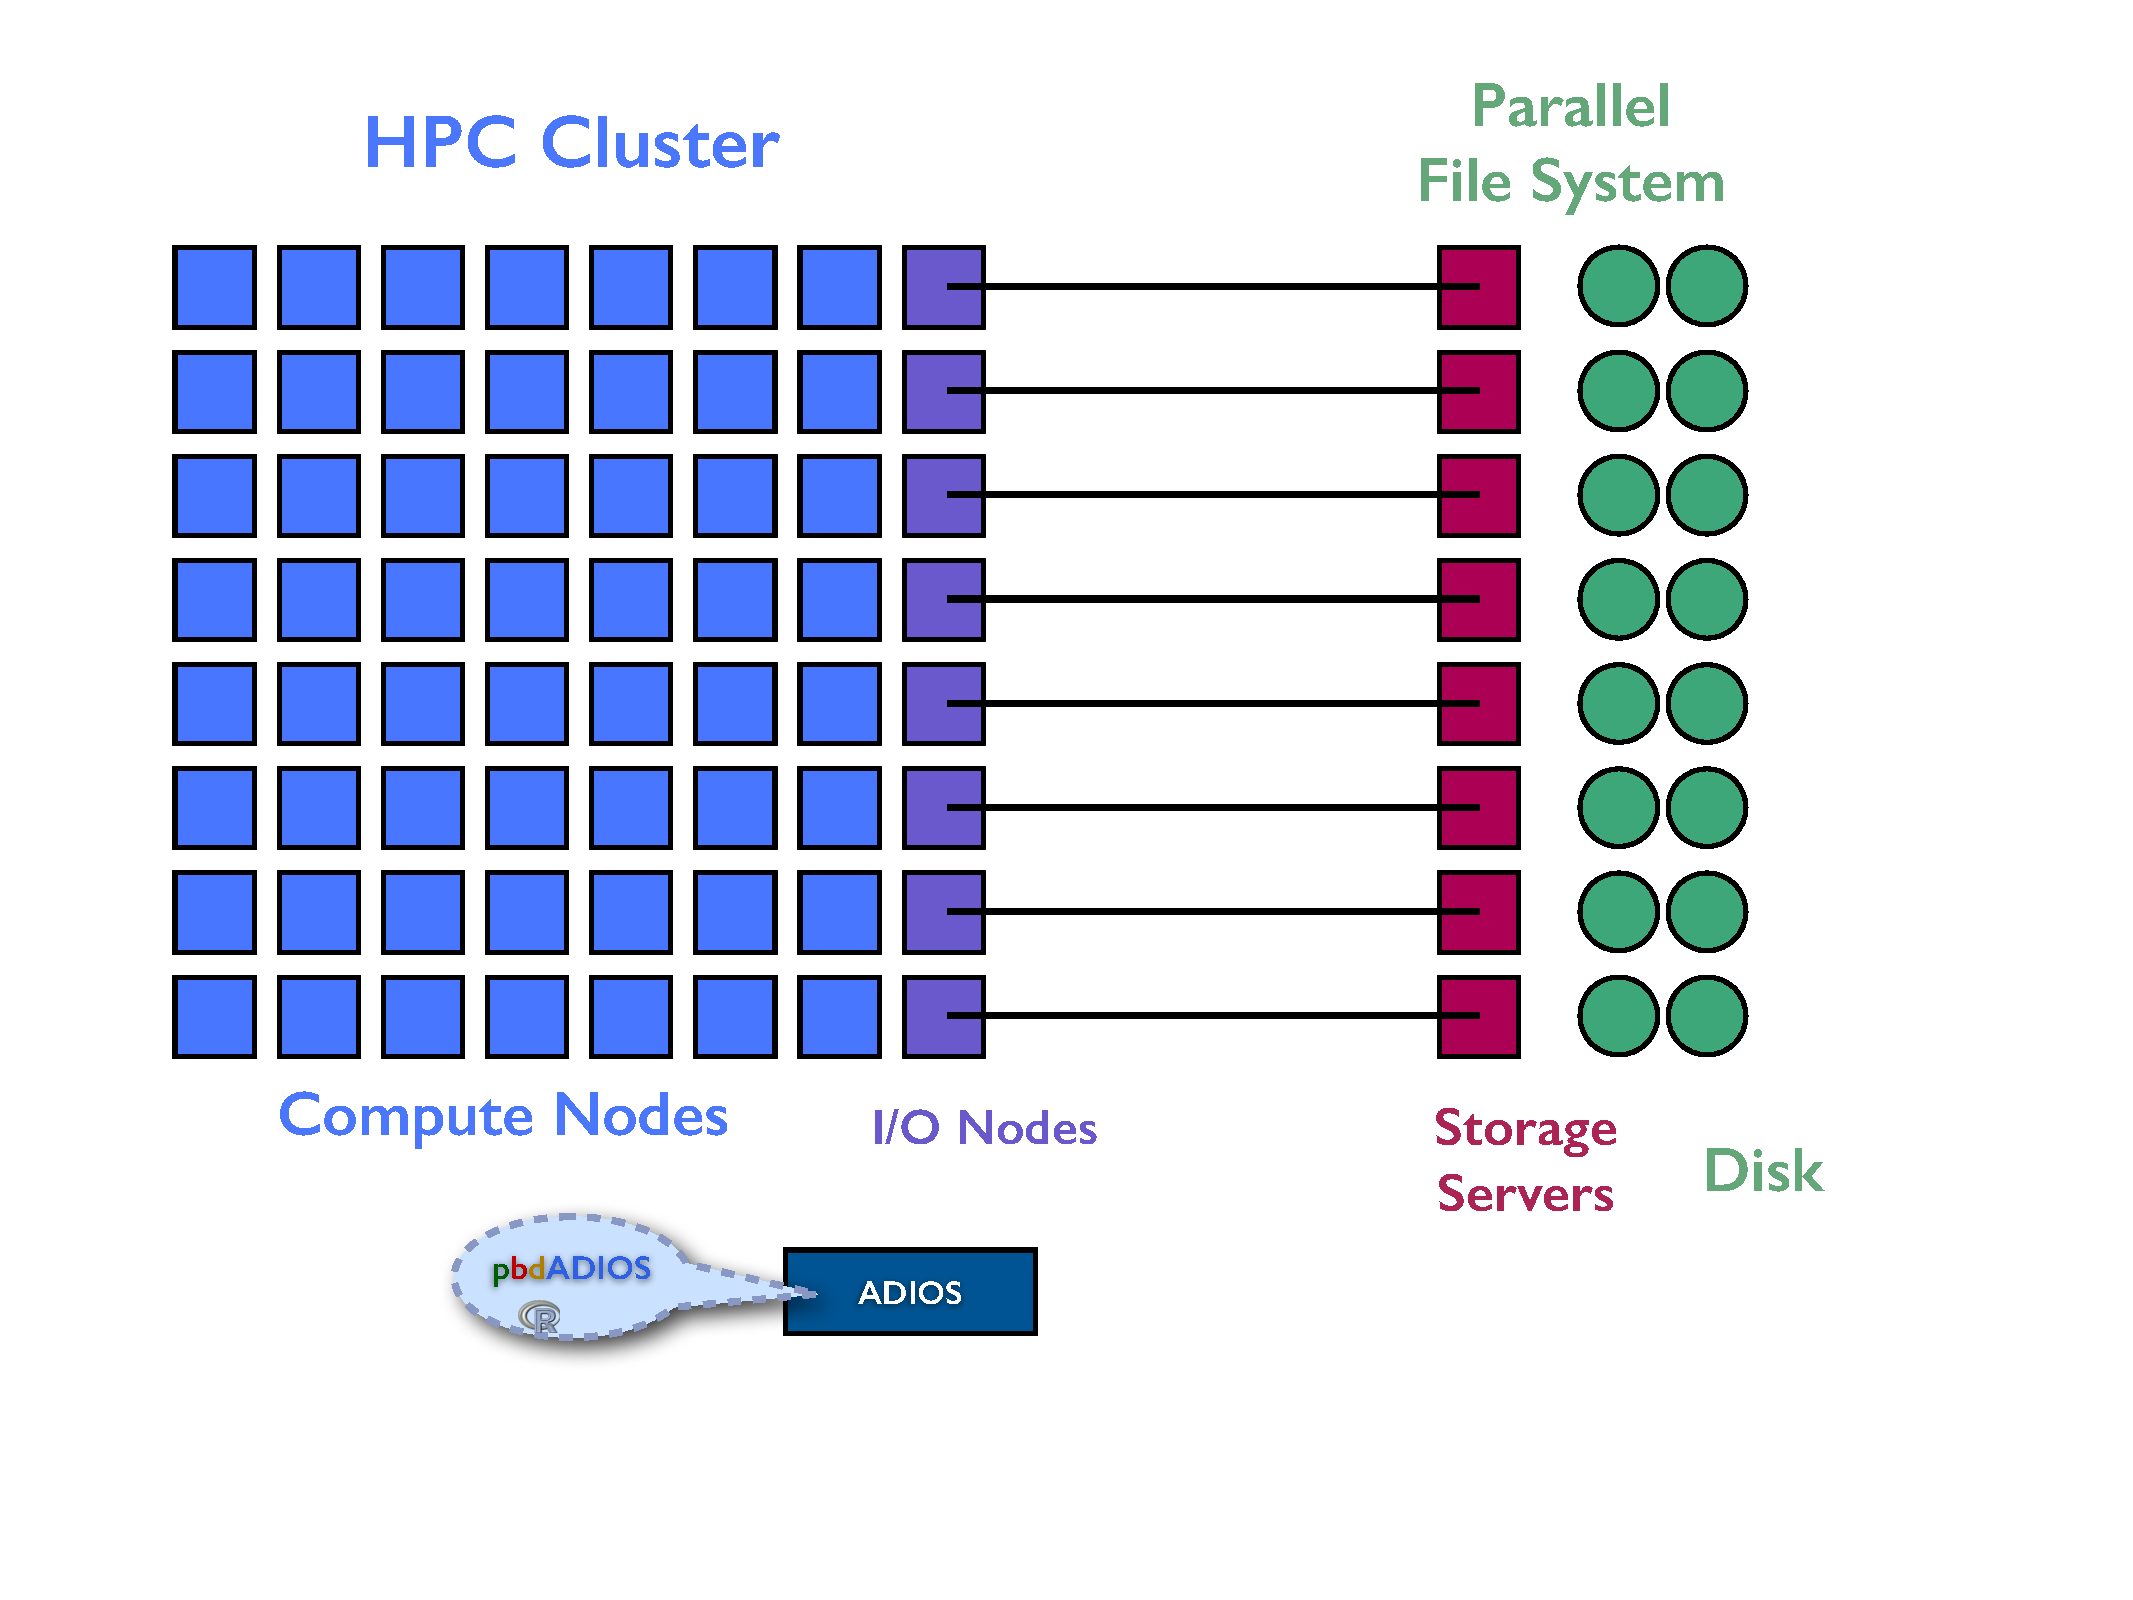
\includegraphics[trim=0 120 30 40,clip,width=1\textwidth]{../common/pics/hardware/ParallelHardware20.pdf}
    \end{block}
  \end{minipage}\hspace{1ex}
  \begin{minipage}{0.32\textwidth}
    \begin{block}{Good.}
      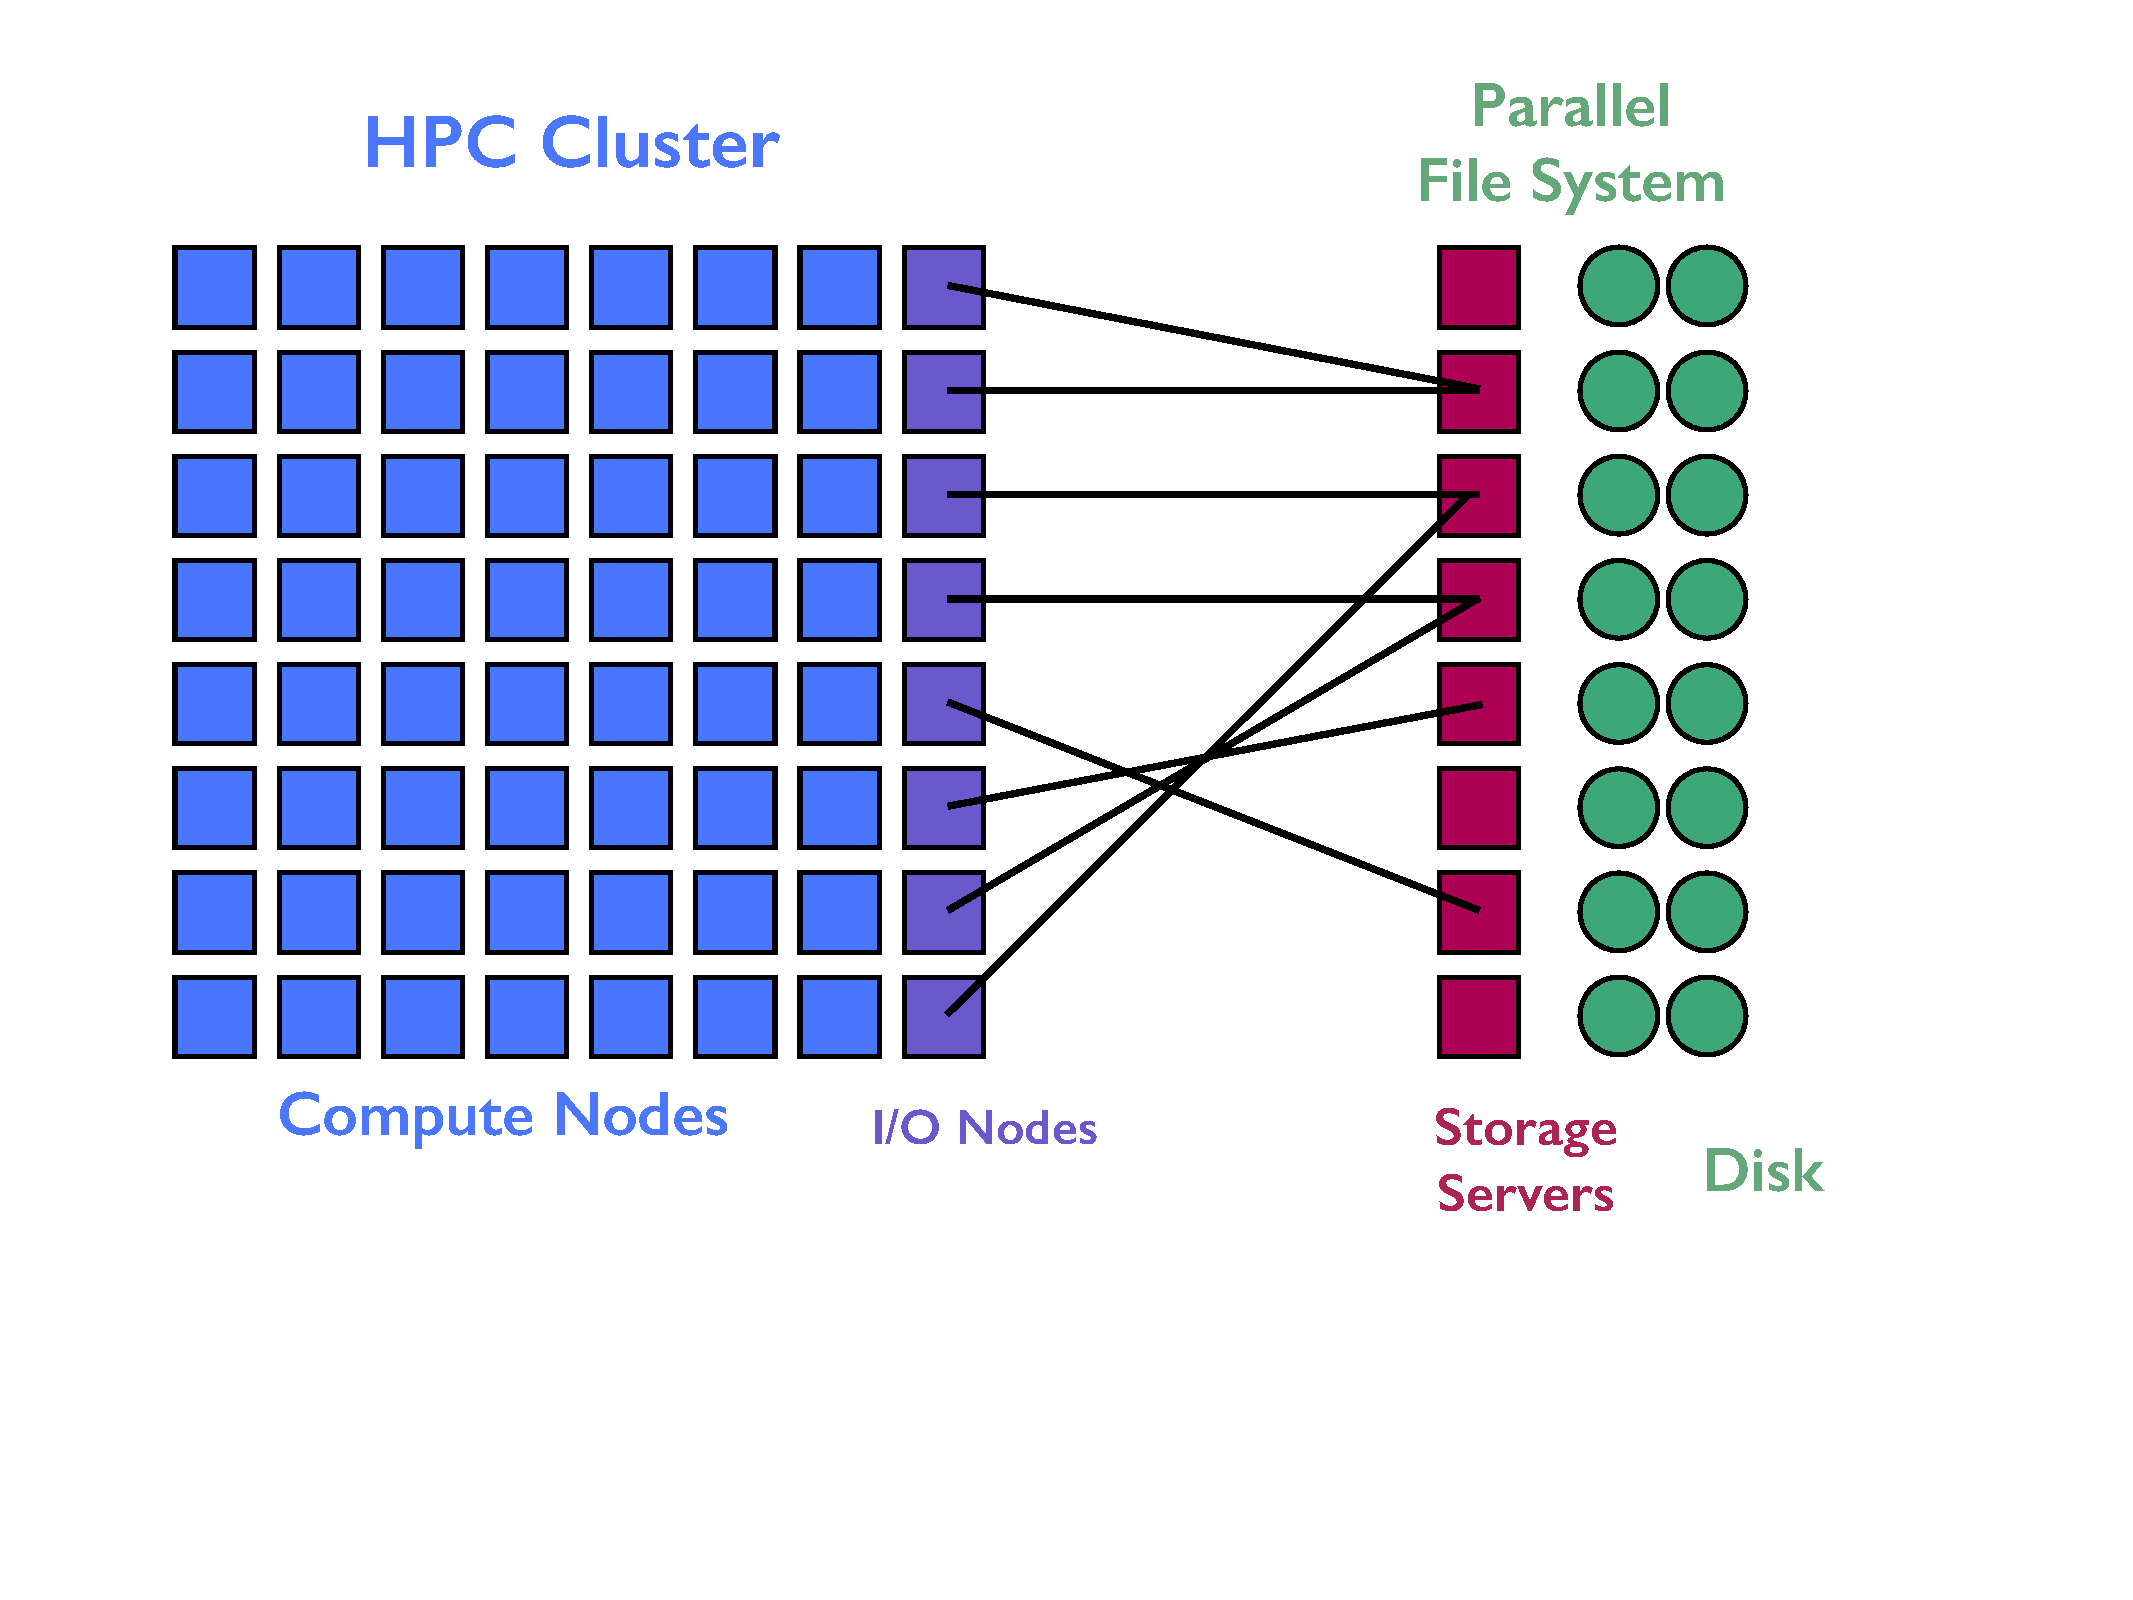
\includegraphics[trim=0 120 30 40,clip,width=1\textwidth]{../common/pics/hardware/ParallelHardware19.pdf}
    \end{block}
  \end{minipage}\hspace{1ex}
  \begin{minipage}{0.32\textwidth}
    \begin{block}{If you have to.}
      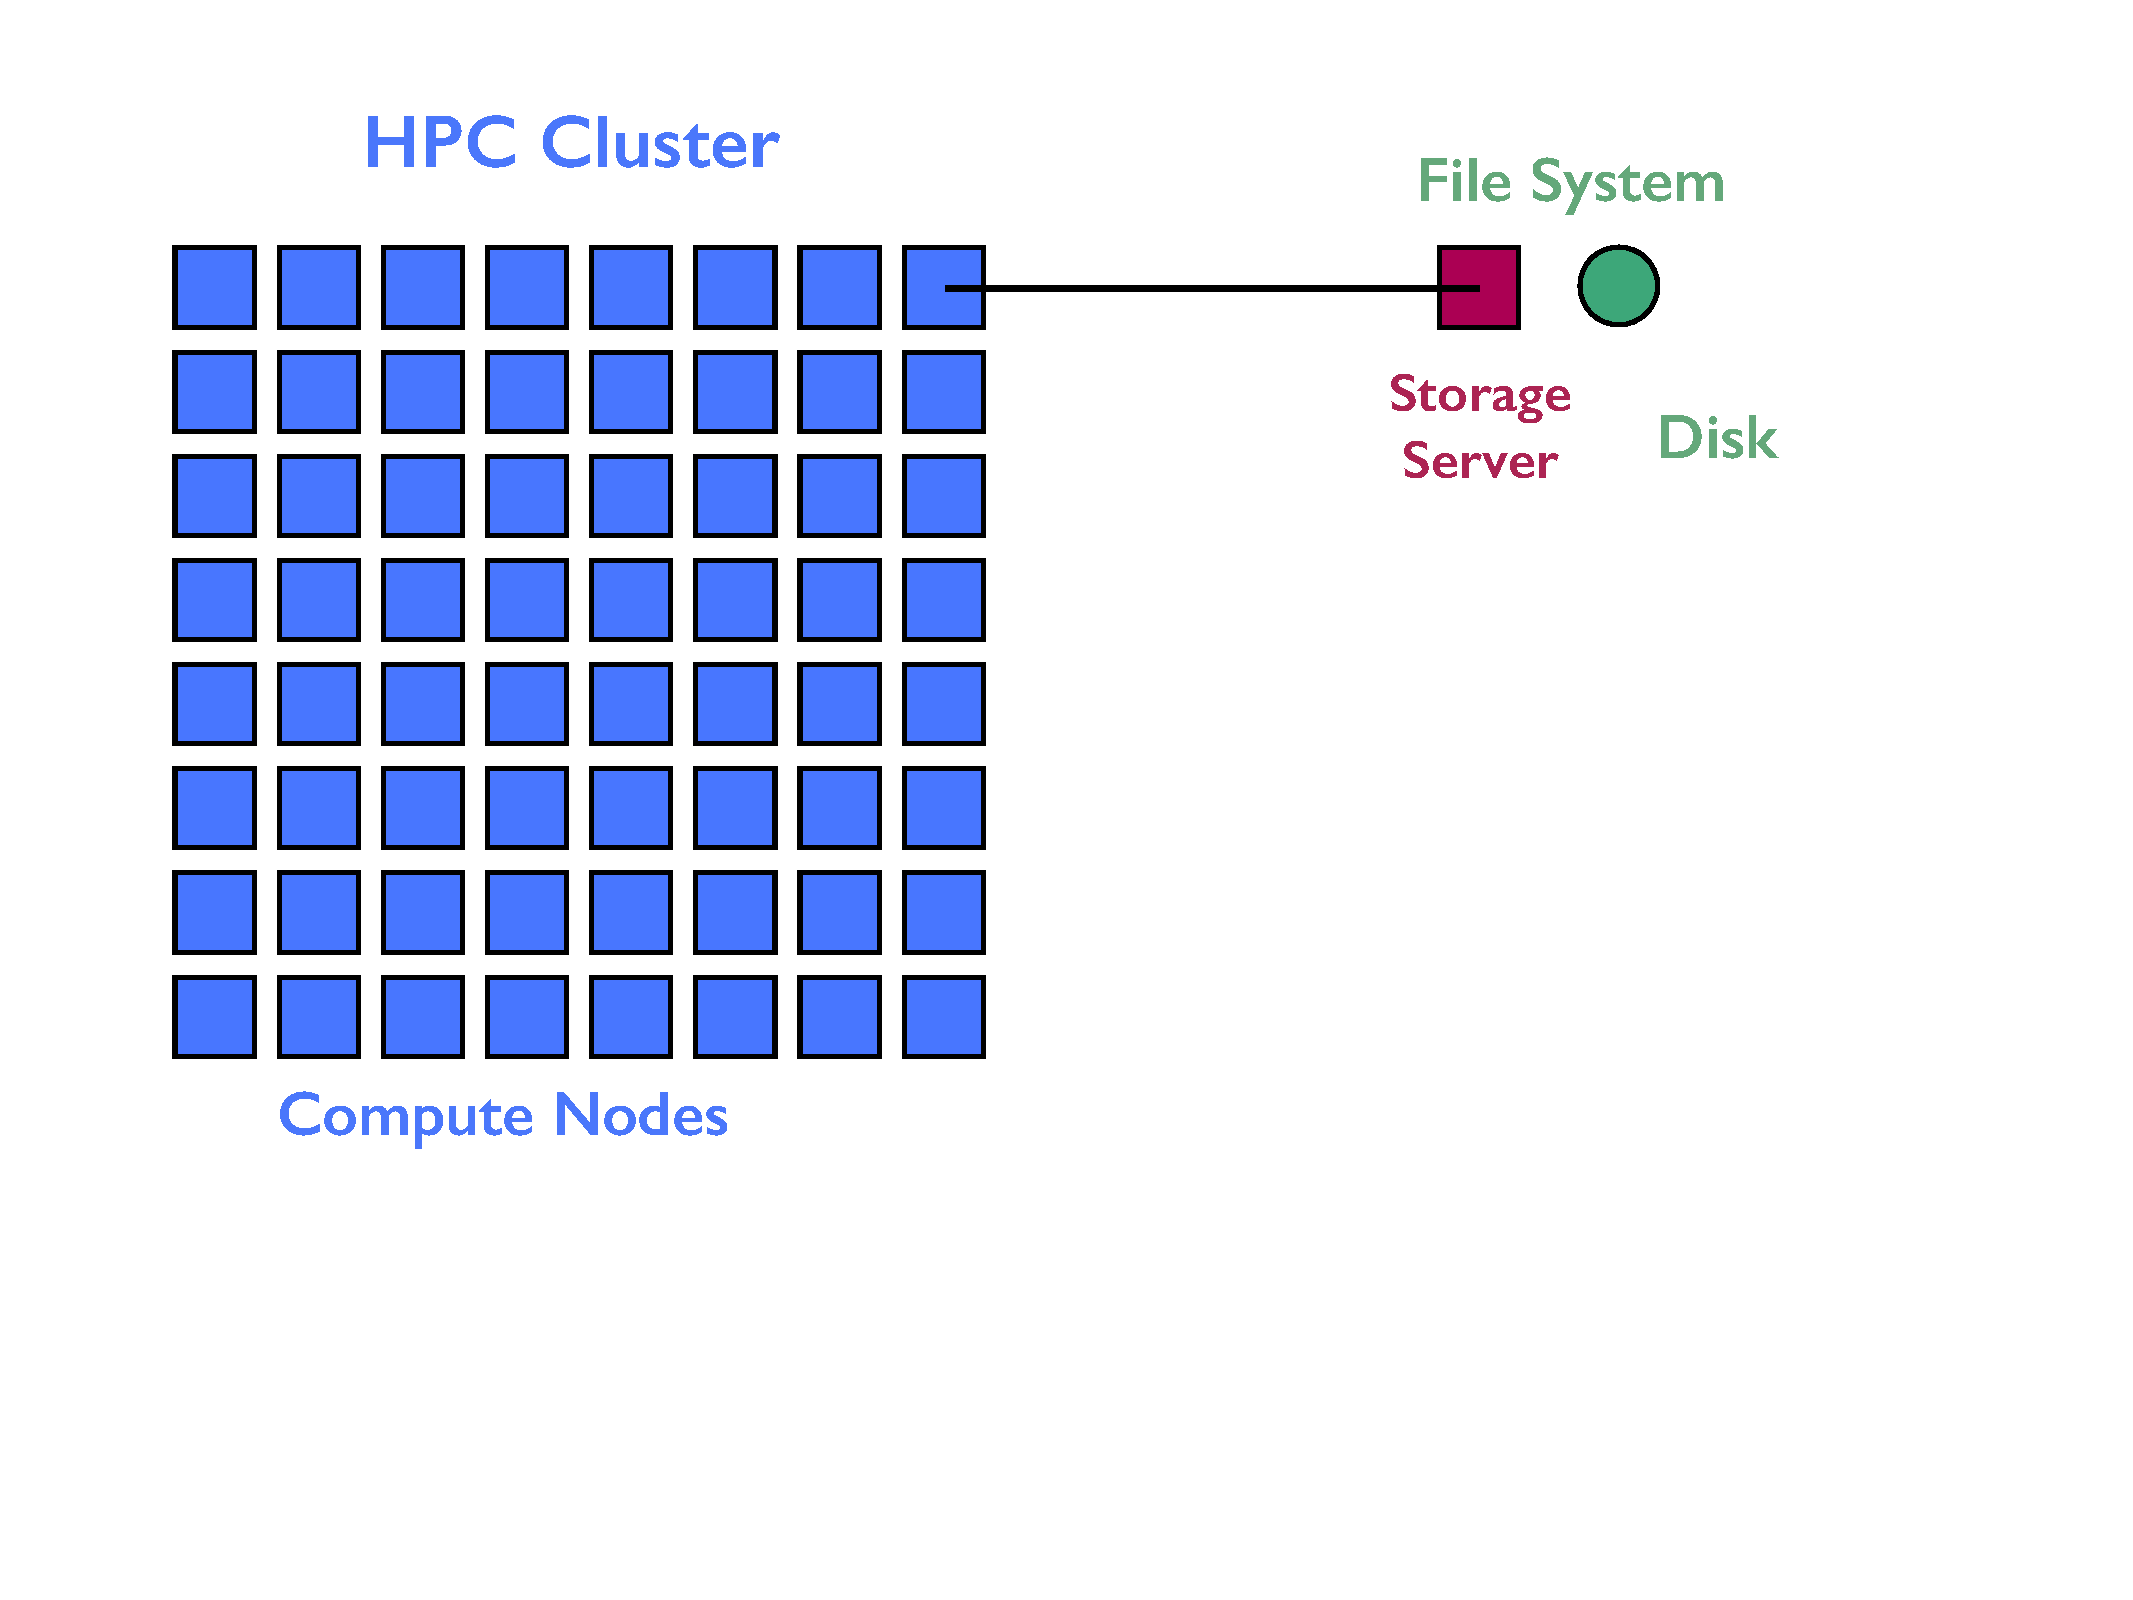
\includegraphics[trim=0 120 30 40,clip,width=1\textwidth]{../common/pics/hardware/ParallelHardware15.pdf}
    \end{block}
  \end{minipage}
  \begin{minipage}{0.32\textwidth}
    \begin{block}{Can work.}
      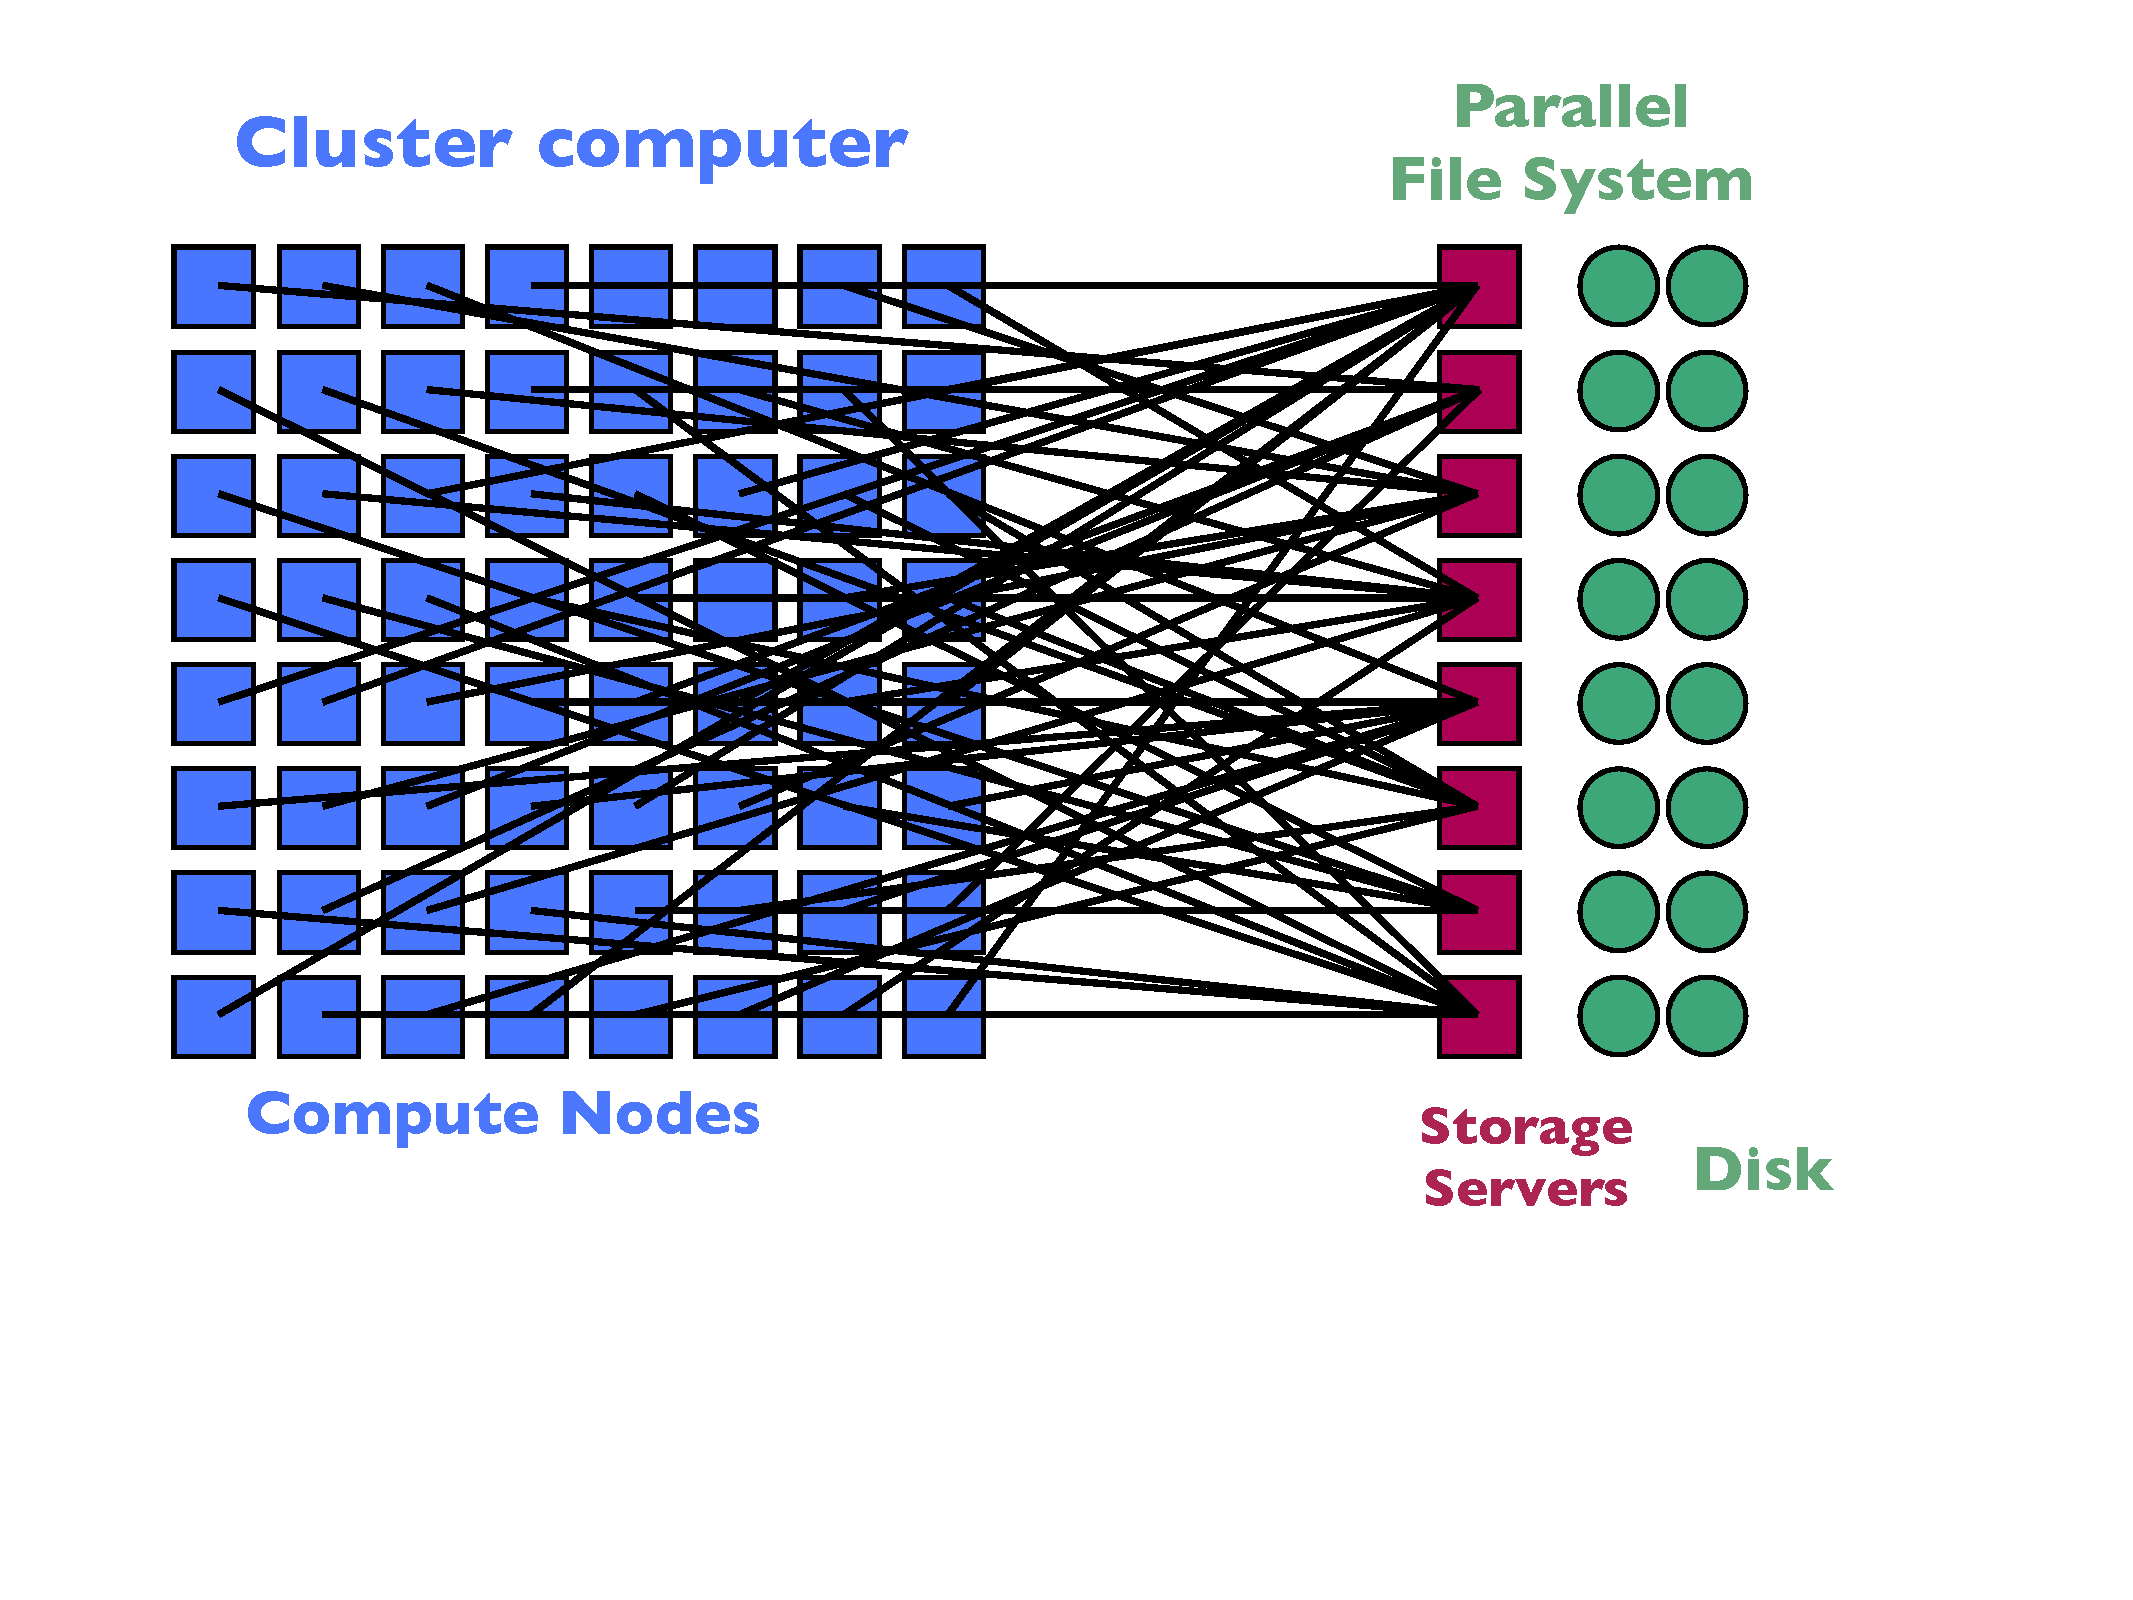
\includegraphics[trim=0 120 30 40,clip,width=1\textwidth]{../common/pics/hardware/ParallelHardware18.pdf}
    \end{block}
  \end{minipage}\hspace{1ex}
  \begin{minipage}{0.32\textwidth}
    \begin{block}{Don't do this!}
      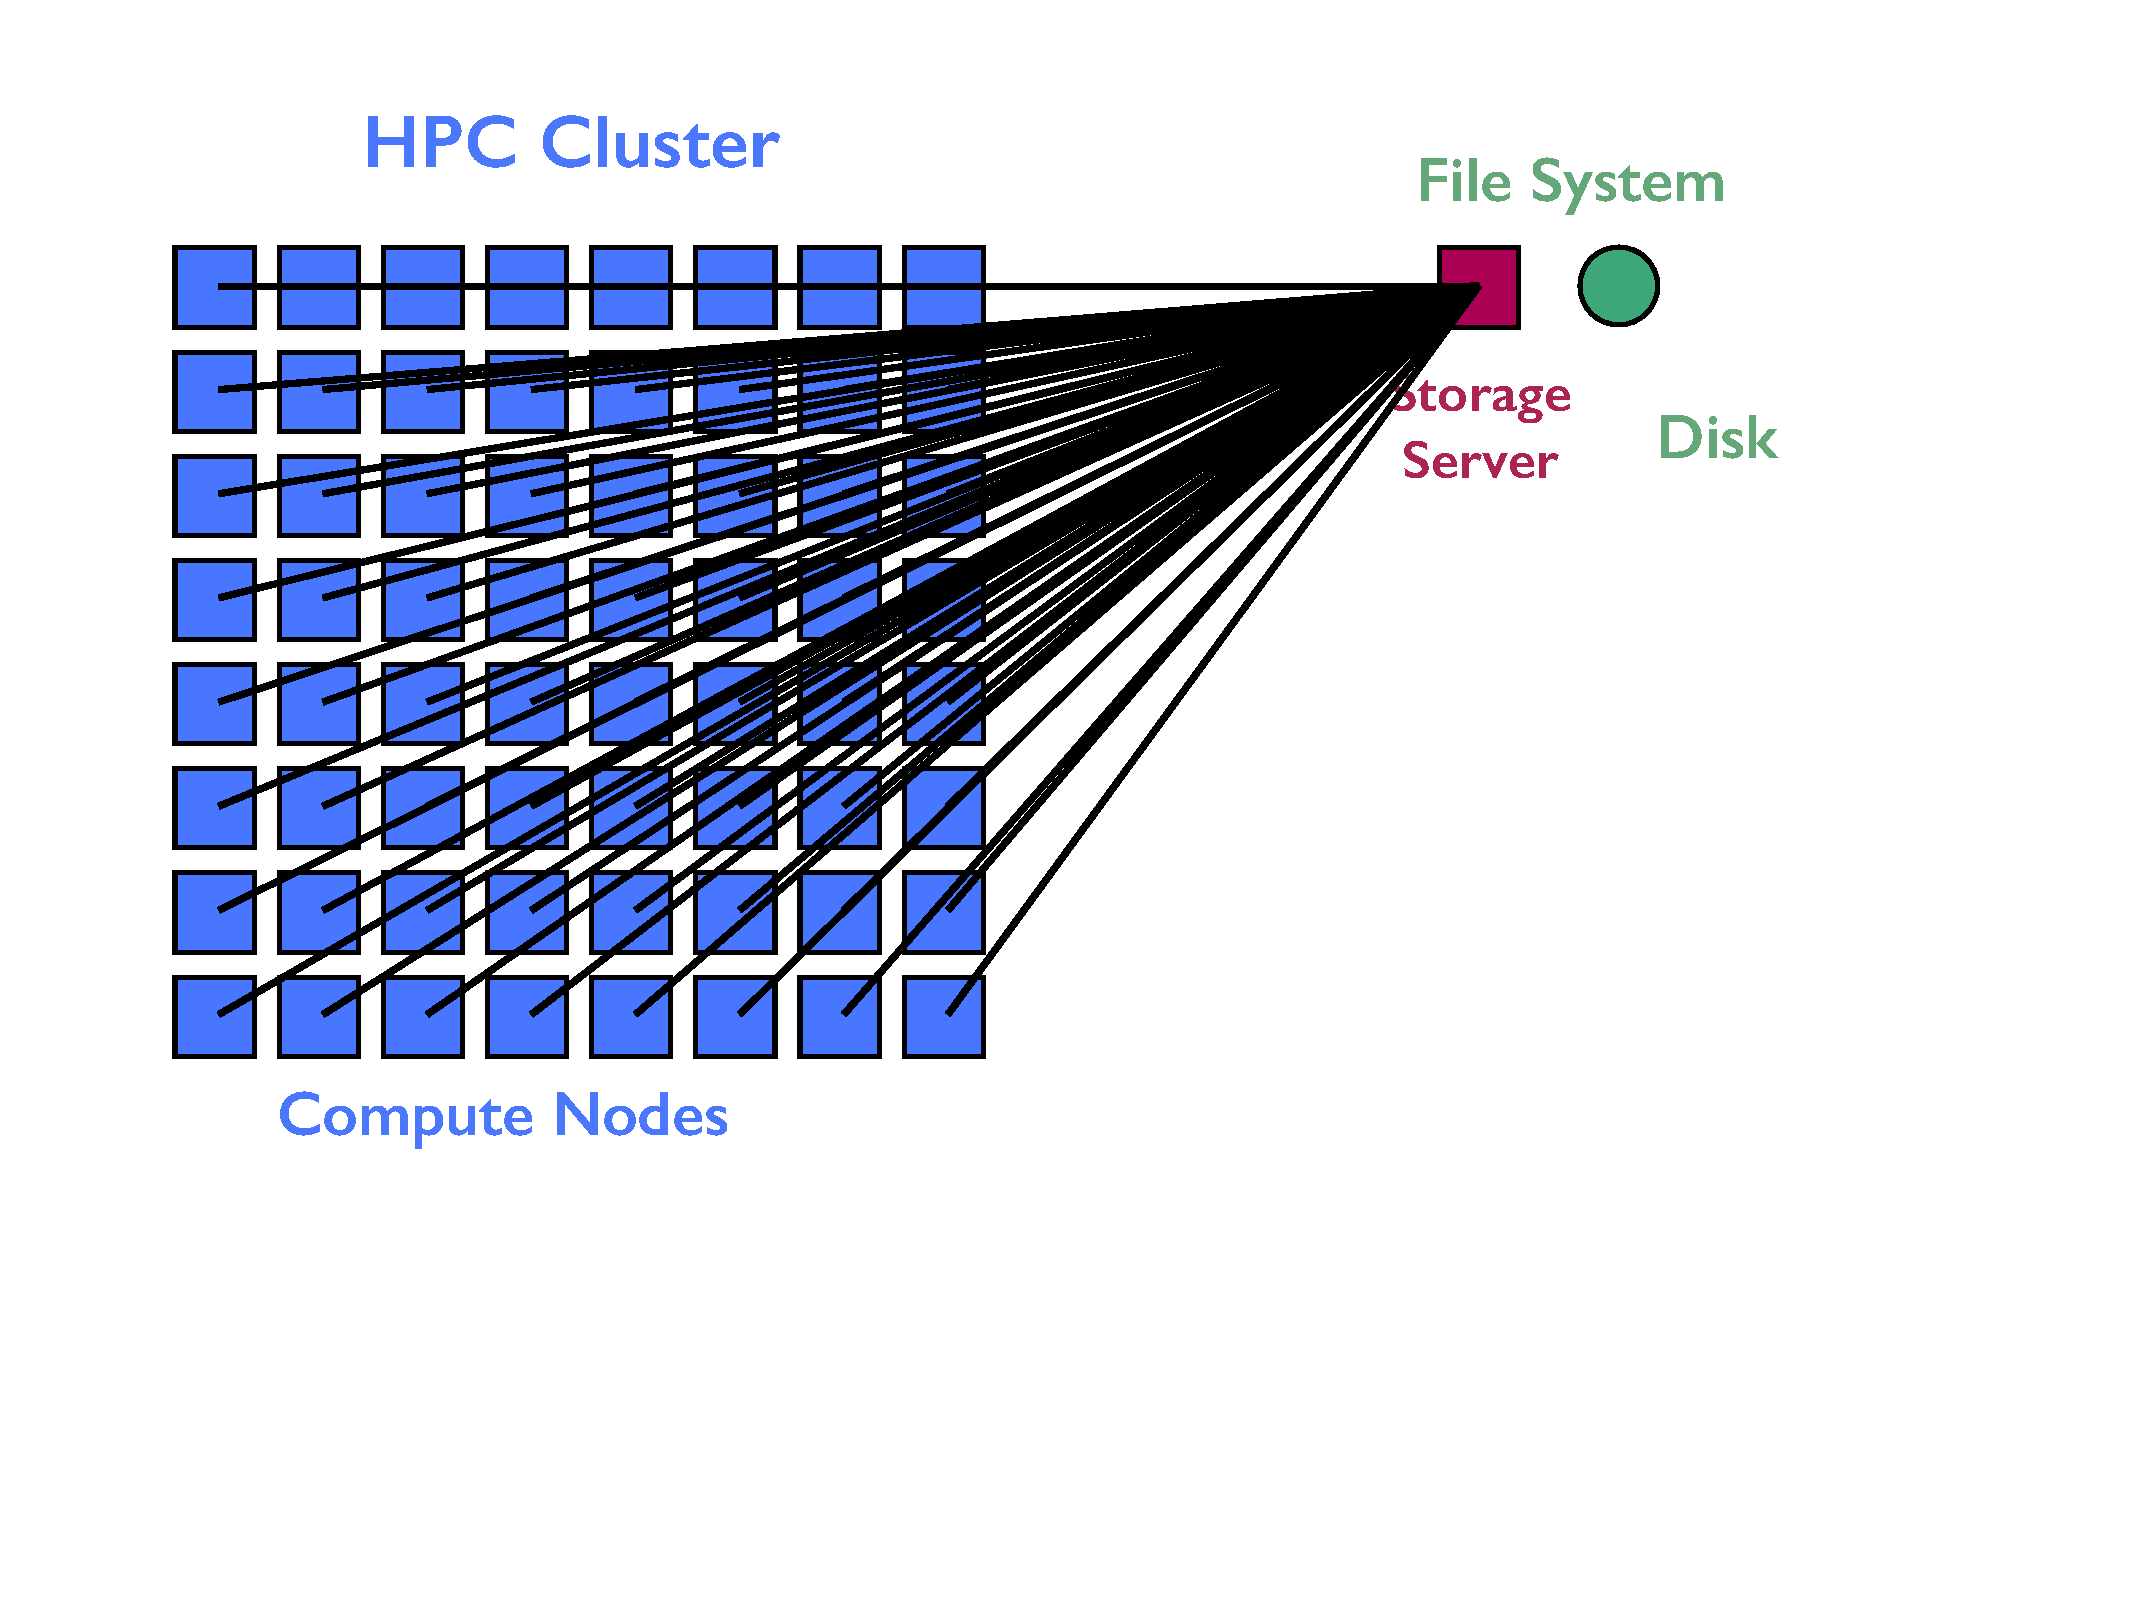
\includegraphics[trim=0 120 30 40,clip,width=1\textwidth]{../common/pics/hardware/ParallelHardware16.pdf}
    \end{block}
  \end{minipage}
\end{frame}

\begin{frame}[fragile]
  \begin{exampleblock}{Matrix in a single large CSV file}\pause
\begin{lstlisting}[title=Serial Code]
x <- read.csv("x.csv")

## rest of your code
\end{lstlisting}

\begin{lstlisting}[title=Partially Parallel Code]
library(pbdDEMO, quiet = TRUE)
init.grid()

dx <- read.csv.ddmatrix("x.csv", header=TRUE, sep=",", 
          nrows=10, ncols=10, num.rdrs=2, ICTXT=0)

## rest of your code

finalize()
\end{lstlisting}
  \end{exampleblock}
\end{frame}

\begin{frame}[fragile]
  \begin{exampleblock}{Matrix in a large binary file (column major)}\pause \vspace{-0.8ex}
    \begin{lstlisting}[title=Parallel Code]
size <- 8 # bytes

my_ids <- get.jid(ncol) # which columns am I reading?
my_ncol <- length(my_ids)
my_start <- (my_ids[1] - 1)*nrow*size
my_length <- my_ncol*nrow

con <- file("binary.matrix.file", "rb")
seekval <- seek(con, where=my_start, rw="read")
x <- readBin(con, what="double", n=my_length, size=size)

gdim <- c(nrow, ncol)
ldim <- c(nrow, my_ncol)
bldim <- c(nrow, allreduce(my_ncol, op="max"))
X <- new("ddmatrix", Data=matrix(x, nrow, my_ncol), dim=gdim, ldim=ldim, bldim=bldim, ICTXT=1)    # glue together as column-block ddmatrix

X <- redistribute(X, bldim=c(2, 2), ICTXT=0)  # redistribute as block-cyclic
Xprc <- prcomp(X)   # proceed as with serial code
    \end{lstlisting}
  \end{exampleblock}
\end{frame}
